%*************************************************
% In this file the first few pages are typeset.
% Make the changes accordingly
%*************************************************

% شماره صفحات با حروف
\pagenumbering{adadi}

%***************************
% 1st page: Blank
%***************************
\thispagestyle{empty}
\mbox{}
\pagebreak

%***************************
% 2nd page: Besmelah
%***************************
\thispagestyle{empty}
\begin{center}
	~\vfill
	
\includegraphics[scale=1]{besm1.jpg}
	~\vfill
\end{center}
\pagebreak

%***************************
% 3rd page: Title
%***************************
\thispagestyle{empty}
%\pagenumbering{gobble}
\newgeometry{left=3cm,right=3cm,top=2cm}
\begin{center}
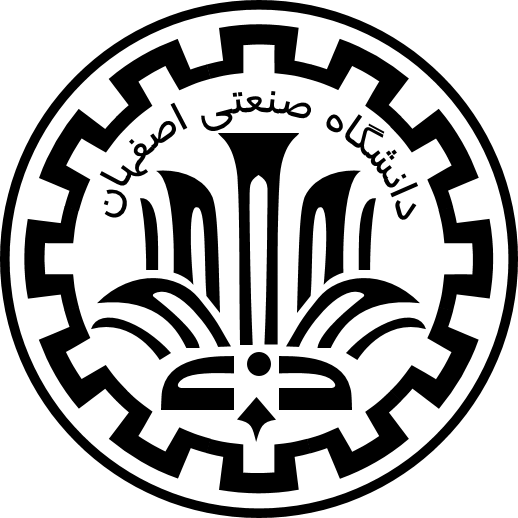
\includegraphics[height=3cm]{iut_logo.png}
\vspace{0.4cm}

\textbf{دانشگاه صنعتی اصفهان}\\
\vspace{0.4cm}

{\large

	دانشکده مهندسی برق و کامپیوتر
}
\vspace{3.5cm}

{\Large
	\textbf{بررسی راه‌های افزایش بهره‌وری در سیستم‌های با بهره‌وری پایین}\\
}
\vspace{3.5cm}

{\Large
	پایان‌نامه کارشناسی ارشد مهندسی برق -- کنترل\\
}
\vspace{1cm}

{\large
	\textbf{آذین آزاده}\\
}
\vspace{3.5cm}

{\large
	استاد راهنما\\
}
\vspace{0.5cm}

{\large
	\textbf{دکتر بهرام برزو}\\
}
\vspace{4cm}

\textbf{1394}

\end{center}
\restoregeometry
\pagebreak

%***************************
% 4th page: Signatures
%***************************
\thispagestyle{empty}
\newgeometry{left=3cm,right=3cm,top=2cm}
\begin{center}
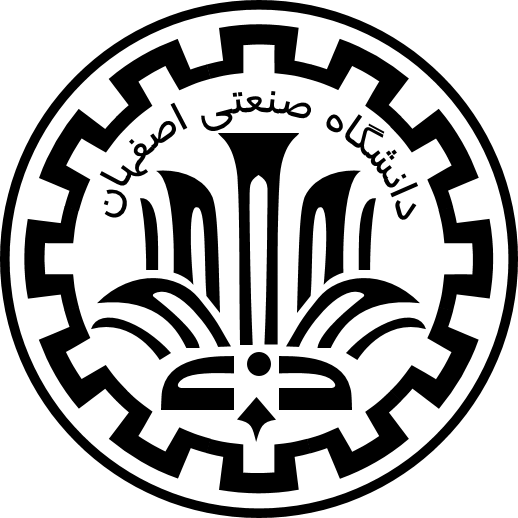
\includegraphics[height=3cm]{iut_logo.png}
\vspace{0.4cm}

\textbf{دانشگاه صنعتی اصفهان}\\
\vspace{0.4cm}

{\large
	دانشکده مهندسی برق و کامپیوتر
}
\vspace{1.8cm}

\vfill

{\Large
	پایان‌نامه کارشناسی ارشد رشته مهندسی برق -- کنترل خانم آذین آزاده\\
	\vspace{.3cm}
	تحت عنوان\\
}


\end{center}
\vfill
\vspace{2.5cm}

{\large
	\textbf{بررسی راه‌های افزایش بهره‌وری در سیستم‌های با بهره‌وری پایین}
}

\vspace*{2cm}

در تاریخ 1394/1/1 توسط کمیته تخصصی زیر مورد بررسی و تصویب نهایی قرار گرفت:\\
\vspace{0.8cm}

{\normalsize
	
	\begin{tabular}{rr}
	\vspace*{.8cm}
	1- استاد راهنمای پایان‌نامه  & \hspace{2cm} دکتر بهرام برزو \\
	\vspace{.8cm}
	2- استاد مشاور پایان‌نامه  &\hspace{2cm} دکتر پوریا پرنیانی \\
	\vspace{.8cm}
	3-استاد داور (اختیاری) &\hspace{2cm} دکتر تهمتن ترابی \\
	\vspace{.8cm}
	۴-استاد داور (اختیاری) &\hspace{2cm} دکتر ثریا ثنایی\\
	\vspace{.8cm}
	سرپرست تحصیلات تکمیلی دانشکده &\hspace{2cm} دکتر جمشید جهانگیر\\
	\end{tabular}
}
\restoregeometry
\pagebreak

%***************************
% 5th page: Acknowledgment
%***************************
\thispagestyle{empty}
\newgeometry{left=3cm,right=4cm,top=4cm}
\vspace*{1.5cm}

{\large
	\textbf{تشکر و قدردانی}\\

	
پروردگار منّان را سپاسگزارم ......

}
\restoregeometry
\pagebreak

%***************************
% 6th page: Rights
%***************************
\thispagestyle{empty}
\newgeometry{left=6cm,right=6cm}

\begin{spacing}{3}
\leavevmode
\vfill
\parbox{8 cm}{

\textbf{\Large کلیه حقوق مادی مترتب بر نتایج مطالعات، ابتکارات و نوآوری‌های ناشی از تحقیق موضوع این پایان‌نامه  متعلق به دانشگاه صنعتی اصفهان است.}

}
\vfill
\end{spacing}
\restoregeometry
\pagebreak

%***************************
% 7th page: Dedication
%***************************
\thispagestyle{empty}
\vspace*{4cm}

{\LARGE
\centering
\textbf{تقدیم به \\ پدر و مادر عزیزم }

}
\pagebreak

%***************************
% 8th page: Table of contents
%***************************

\titleformat{\chapter}[display]
	{\normalfont\LARGE\bfseries\centering}{\chaptertitlename ~ \tartibi{chapter}}{20pt}{\LARGE}
\newgeometry{left=2.5cm,right=3cm,top=3cm,bottom=2.5cm,includehead=false,headsep=1cm,footnotesep=.5cm}
\baselineskip=.7cm

\addtocontents{toc}{\textbf{\underline{عنوان}}}
\addtocontents{toc}{\hfill\textbf{\underline{صفحه}}\par}
\addcontentsline{toc}{section}{فهرست مطالب}
\tableofcontents
\pagebreak

\addcontentsline{toc}{section}{فهرست تصاویر}
\listoffigures
\pagebreak

%\addcontentsline{toc}{section}{فهرست جداول}
%\listoftables
%\pagebreak

% change the font and margins of a chapter title
\titlespacing*{\chapter}{0pt}{3.5cm}{6cm}
\titleformat{\chapter}[display]
	{\normalfont\LARGE\bfseries\raggedright}{\chaptertitlename ~ \tartibi{chapter}}{20pt}{\LARGE}

% No page numbers on the first page of a chapter
\assignpagestyle{\chapter}{empty}
